% \date{May 14, 2024}
% \author{Deralive}
% \title{华东师范大学软件学院实验报告模板}
% 注意事项:编译两次,以确保目录、页码完整显示

\def\allfiles{}

%————————————多文件编译————————————%
% \ifx\allfiles\undefined
% 	    \begin{document}
% \else
% \fi

% Content

% \ifx\allfiles\undefined
% 	    \end{document}
% 	\else
% 	\fi
%—————————————————————————————————%

\documentclass[14pt,a4paper,UTF8,twoside]{article}

\usepackage{amsmath}
\usepackage{graphicx}
\usepackage{geometry} 
\usepackage{ctex}
\usepackage{booktabs} % 表格库
\usepackage{titlesec} % 标题库
\usepackage{fancyhdr} % 页眉页脚库
\usepackage{lastpage} % 页码数库
\usepackage{listings} % 代码块包
\usepackage{xcolor}
\usepackage[hidelinks]{hyperref}
\usepackage{tikz}
\usepackage{tikz-qtree}
\usepackage{fontspec} % 允许设置字体
\usepackage{unicode-math} % 允许数学公式使用特定字体
\usepackage{mwe}
\usepackage{zhlipsum} % 中文乱数文本
\usepackage{amsmath}
\usepackage{xcolor}
\usepackage{float} % 浮动体环境
\usepackage{subcaption} % 子图包
\usepackage{biblatex}
\addbibresource{references.bib} % 指定你的.bib文件名称

\definecolor{mygreen}{rgb}{0,0.6,0}
\definecolor{mygray}{rgb}{0.5,0.5,0.5}
\definecolor{mymauve}{rgb}{0.58,0,0.82}

\date{} % 留空,以让编译时去除日期

%———————————————注意事项—————————————————%

% 1、如果编译显示失败,但没有错误信息,就是 filename.pdf 正在被占用
% 2、在文件夹中的终端使用 Windows > xelatex filename.tex 也可编译

%—————————————华东师范大学———————————————%

% 论文制作时须加页眉,页眉从中文摘要开始至论文末
% 偶数页码内容为:华东师范大学硕士学位论文,奇数页码内容为学位论文题目

%————————定义 \section 的标题样式————————%

% 注意:\chapter 等命令,内部使用的是 \thispagestyle{plain} 的排版格式
% 若需要自己加上页眉,实际是在用 \thispagestyle{fancy} 的排版格式
% 加上下面这一段指令,就能够让 \section 也使用 fancy 的排版格式
% 本质就是让目录、第一页也能够显示页眉、页脚

\fancypagestyle{plain}{
  \pagestyle{fancy}
}

\title{华东师范大学软件学院课程作业} % 模板
\titleformat{\section}
    {\normalfont\bfseries\Large} % 字体大小、字体系列(\bfseries 为加粗)
    {\thesection}{1em}{}

% 设置章节的中文格式
\renewcommand\thesection{\chinese{section} \hspace{0pt}}
\renewcommand\thesubsection{\arabic{subsection} \hspace{0pt}}
% \renewcommand\thesubsubsection{\alph{subsubsection} \hspace{0pt}} % 字母编号
% \hspace{0pt} 是为了确保在章节编号和章节题目之间不要有空格,使得排版更为美观
    
%—————————————页面基础设置———————————————%

\geometry{left=10mm, right=10mm, top=20mm, bottom=20mm}

%————————————设置页眉、页脚——————————————%

\pagestyle{fancy} % 设置 plain style 的属性

% 设置页眉

\fancyhead[RE]{\leftmark} % Right Even 偶数页右侧显示章名 \leftmark 最高级别章名
\fancyhead[LO]{\rightmark} % Left Odd 奇数页左侧显示节名 \rightmark 第二级别节名
\fancyhead[C]{华东师范大学软件学院课程作业} % Center 居中显示
\fancyhead[LE,RO]{~\thepage~} % 在偶数页的左侧,奇数页的右侧显示页码
\renewcommand{\headrulewidth}{1.2pt} % 页眉与正文之间的水平线粗细

% 设置页脚:在每页的右下脚以斜体显示书名

\fancyfoot[RO,RE]{\it Lab Report By \LaTeX} % 使用意大利斜体显示
\renewcommand{\footrulewidth}{0.5pt} % 页脚水平线宽度

% 设置页码:在底部居中显示页码

\pagestyle{fancy}
\fancyfoot[C]{\kaishu 第 \thepage 页 \ 共 \pageref{LastPage} 页} % LastPage 需要二次编译以获取总页数

%——————————————代码块设置———————————————%

\lstset {
    backgroundcolor=\color{white},   % choose the background color; you must add \usepackage{color} or \usepackage{xcolor}
    basicstyle=\footnotesize,        % the size of the fonts that are used for the code
    breakatwhitespace=false,         % sets if automatic breaks should only happen at whitespace
    breaklines=true,                 % sets automatic line breaking
    captionpos=bl,                   % sets the caption-position to bottom
    commentstyle=\color{mygreen},    % comment style
    deletekeywords={...},            % if you want to delete keywords from the given language
    escapeinside={\%*}{*},           % if you want to add LaTeX within your code
    extendedchars=true,              % lets you use non-ASCII characters; for 8-bits encodings only, does not work with UTF-8
    frame=single,                    % adds a frame around the code
    keepspaces=true,                 % keeps spaces in text, useful for keeping indentation of code (possibly needs columns=flexible)
    keywordstyle=\color{blue},       % keyword style
    % language=Python,               % the language of the code
    morekeywords={*,...},            % if you want to add more keywords to the set
    numbers=left,                    % where to put the line-numbers; possible values are (none, left, right)
    numbersep=5pt,                   % how far the line-numbers are from the code
    numberstyle=\tiny\color{mygray}, % the style that is used for the line-numbers
    rulecolor=\color{black},         % if not set, the frame-color may be changed on line-breaks within not-black text (e.g. comments (green here))
    showspaces=false,                % show spaces everywhere adding particular underscores; it overrides 'showstringspaces'
    showstringspaces=false,          % underline spaces within strings only
    showtabs=false,                  % show tabs within strings adding particular underscores
    stepnumber=1,                    % the step between two line-numbers. If it's 1, each line will be numbered
    stringstyle=\color{orange},      % string literal style
    tabsize=2,                       % sets default tabsize to 2 spaces
    % title=Python Code              % show the filename of files included with \lstinputlisting; also try caption instead of title
}

% 注释掉的部分用于后续插入代码,参数可调整,格式如下:

% 1、直接插入
% \begin{lstlisting}[language = ? , title = { ? } ]
%       Your code here.
% \end{lstlisting}

% 2、文件插入
% \lstinputlisting[language = C , title = ?.c] {filename.c}

%———————————————字体设置————————————————%

% \setCJKmainfont{SimSun} % 设置正文罗马族的 CJK 字体
% \renewcommand{\normalsize}{\fontsize{12pt}{15pt}\selectfont} % 设置正文字号
\linespread{1.2}

%——————————————————————————————————————%

%———————————————超链接设置——————————————%

\hypersetup{
    pdfstartview=FitH, % 设置PDF文档打开时的初始视图为页面宽度适应窗口宽度(即页面水平适应)
    CJKbookmarks=true, % 用对CJK(中文、日文、韩文)字符的书签支持,确保这些字符在书签中正确显示
    bookmarksnumbered=true, % 书签带有章节编号。这对有章节编号的文档很有用
    bookmarksopen=true, % 文档打开时,书签树是展开的,方便查看所有书签
    colorlinks, % 启用彩色链接。这样,链接在PDF中会显示为彩色,而不是默认的方框
    pdfborder=001, % 设置PDF文档中链接的边框样式。001 表示链接周围没有边框,仅在单击时显示一个矩形
    linkcolor=blue, % 设置文档内部链接(如目录中的章节链接)的颜色为蓝色
    anchorcolor=blue, % 设置锚点链接(即目标在同一文档内的链接)的颜色为蓝色
    citecolor=blue, % 设置引用(如文献引用)的颜色为蓝色
}

%——————————————导言区结束,进入正文部分———————————————%

%——————————————————————————————————————%

\begin{document}

\maketitle

\begin{center} % \extracolsep{\fill} 拉伸到页面最大宽度前,保证居中显示

  \begin{tabular*}{\textwidth}{@{\extracolsep{\fill}} l  l  l }
    \hline
    课程名称:计算机网络 &  年级:2023级本科  &  姓名:张梓卫 \\
    作业主题:第四章作业 & 学号:10235101526 & 作业日期:2024/12/03 \\
    指导老师:刘献忠 & 组号: \\
    \hline
  \end{tabular*}

\end{center}

% \tableofcontents % 目录也需要二次编译

\section{4.1}

\subsection*{题目}
A group of N stations share a 56-kbps pure ALOHA channel. Each station outputs a 1000-bit frame on average once every 100 sec, even if the previous one has not yet been sent (e.g., the stations can buffer outgoing frames). What is the maximum value of N?

\subsection*{解答}

在纯 ALOHA 协议中,信道的可用带宽效率为 18.4\%。给定信道的总带宽为 56 kbps,因此其可用带宽为:
\[
56 \times 0.184 = 10.304 \, \text{kbps}
\]

每个站点平均需要的带宽为 10 bps。因为每个站点每 100 秒发送一个 1000 比特的帧,其平均带宽需求为:
\[
\frac{1000 \, \text{比特}}{100 \, \text{秒}} = 10 \, \text{bps}
\]

因此,信道最多可以支持的站点数目 \(N\) 为:
\[
N = \frac{\text{可用带宽}}{\text{每站点所需带宽}} = \frac{10,304 \, \text{bps}}{10 \, \text{bps}} = 1030 \, \text{站点}
\]

\section{4.2}

\subsection*{题目}
Measurements of a slotted ALOHA channel with an infinite number of users show that 10\% of the slots are idle.

(a) What is the channel load, G?  
(b) What is the throughput?  
(c) Is the channel underloaded or overloaded?

\subsection*{解答}

(a) 计算信道负载 \(G\):

根据泊松分布定理,空闲槽的概率为:
\[
P(k = 0) = e^{-G}
\]

已知 10\% 的槽为空闲,即 \(P(k = 0) = 0.1\),代入公式可得:
\[
e^{-G} = 0.1 \quad \Rightarrow \quad G = -\ln(0.1) = 2.3
\]

因此,信道负载为 \(G = 2.3\)。

\vspace{0.5cm}

(b) 计算吞吐量:

吞吐量 \(S\) 的计算公式为:
\[
S = G \cdot P(k = 0)
\]

代入已知值 \(G = 2.3\) 和 \(P(k = 0) = 0.1\):
\[
S = 2.3 \cdot 0.1 = 0.23
\]

因此,吞吐量为 \(S = 0.23\)。

\vspace{0.5cm}

(c) 判断信道负载状态:

对于时隙 ALOHA,如果 \(G \leq 1\),信道欠载;如果 \(G > 1\),信道过载。

由于 \(G = 2.3 > 1\),则信道过载。

\section{4.3}

\subsection*{题目}
What is the baud rate of classic 10-Mbps Ethernet?

\subsection*{解答}

经典以太网使用曼彻斯特编码,每个比特由两个符号组成,符号速率(baud rate)是比特率的两倍。

给定经典以太网的比特率为 10 Mbps:
\[
\text{符号速率(Baud rate)} = 2 \times \text{比特率(Bit rate)} = 2 \times 10 \, \text{Mbps} = 20 \, \text{Mbaud/s}
\]

\section{4.4}

\subsection*{题目}
Sketch the Manchester encoding on a classic Ethernet for the bit stream 0001110101.

\subsection*{解答}
在经典以太网中,使用曼彻斯特编码,故最终的比特流应为:

\begin{figure}[H]
    \centering
    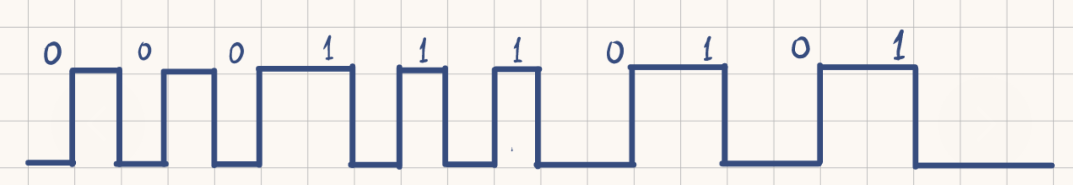
\includegraphics[width=0.5\textwidth]{lec4/manchester.png}
    \caption{Manchester 编码}
    \label{fig:manchester}
\end{figure}

\section{4.5}

\subsection*{题目}
A 1-km-long, 10-Mbps CSMA/CD LAN (not 802.3) has a propagation speed of 200m/μs. Repeaters are not allowed in this system. Data frames are 256 bits long, including 32 bits of header, checksum, and other overhead. The first bit slot after a successful transmission is reserved for the receiver to capture the channel in order to send a 32-bit acknowledgment frame. What is the effective data rate, excluding overhead, assuming that there are no collisions?

\subsection*{解答}
整个传输过程包括六个阶段:
\begin{enumerate}
    \item 发送端占用信道时间:10 毫秒
    \item 传输数据的时间:25.6 毫秒
    \item 最后一位比特到达终端的延迟:5 毫秒
    \item 接收端占用信道时间:10 毫秒
    \item 发送确认帧的时间:3.2 毫秒
    \item 最后一位比特返回发送端的延迟:5 毫秒
\end{enumerate}

将这些时间加总,得到总耗时为:$ 58.8 \, \text{毫秒} $.

在这一时间段内,实际发送的数据位数为 \(224 \, \text{比特}\)。因此,实际有效数据速率为:
\[
\text{有效数据速率} = \frac{224 \, \text{比特}}{58.8 \, \text{毫秒}} = 3.8 \, \text{Mbps}
\]

\section{4.6}

\subsection*{题目}
Consider building a CSMA/CD network running at 1 Gbps over a 1-km cable with no repeaters. The signal speed in the cable is 200,000 km/sec. What is the minimum frame size?

\subsection*{解答}

在 CSMA/CD 协议下,为了检测到碰撞并确保传输正确,帧的传输时间必须大于或等于信号的往返传播时间。最小帧大小的计算基于以下公式:
\[
\frac{L}{B} \geq 2\tau
\]

其中:
\begin{itemize}
    \item \(L\):帧的最小长度,\(B\) 是网络带宽(单位:bps)
    \item \(\tau\):信号的单程传播时间(单位:秒)
\end{itemize}

已知:
\begin{itemize}
    \item 网络长度:\(1 \, \text{km}\),信号传播速度:\(200,000 \, \text{km/s}\),网络带宽:\(1 \, \text{Gbps}\)
\end{itemize}


单程传播时间:
\[
\tau = \frac{\text{网络长度}}{\text{信号传播速度}} = \frac{1 \, \text{km}}{200,000 \, \text{km/s}} = 5 \, \mu\text{s}
\]

往返传播时间:
\[
2\tau = 2 \times 5 \, \mu\text{s} = 10 \, \mu\text{s}
\]

最小帧大小:
根据公式:
\[
\frac{L}{B} \geq 2\tau \quad \Rightarrow \quad L \geq B \times 2\tau
\]

\[
L \geq 1 \, \text{Gbps} \times 10 \, \mu\text{s} = 10,000 \, \text{比特}
\]

\[
L = 10,000 \, \text{比特} = 1,250 \, \text{字节}
\]

\section{4.7}

\subsection*{题目}
Ethernet frames must be at least 64 bytes long to ensure that the transmitter is still going in the event of a collision at the far end of the cable. Fast Ethernet has the same 64-byte minimum frame size but can get the bits out ten times faster. How is it possible to maintain the same minimum frame size?

\subsection*{解答}

在以太网(Ethernet)中,帧的最小长度必须足够大,以确保在发生碰撞时,发送方能够检测到碰撞。其原因在于,CSMA/CD 协议需要在帧传输结束前,信号能够往返于链路两端,只有这样才能保证发生碰撞时,发送方可以及时中止传输并进行重传。

在普通以太网中,帧的最小长度为 64 字节(即 512 比特),这对应于 10 Mbps 的传输速率和最大 2500 米的电缆长度。在这种情况下:
1. 帧传输时间为:
   \[
   \text{帧传输时间} = \frac{\text{帧大小}}{\text{带宽}} = \frac{512 \, \text{比特}}{10 \, \text{Mbps}} = 51.2 \, \mu\text{s}
   \]

2. 信号的往返传播时间(Round Trip Time, RTT)与帧传输时间相匹配,确保在碰撞发生时,发送方仍然处于传输状态。

在快速以太网(Fast Ethernet)中,速率提升到了 100 Mbps,比普通以太网快了 10 倍。然而,最小帧长度仍保持为 64 字节。为了解决传输速率提高导致信号传播时间不足的问题,需要缩短电缆的最大长度,从而使信号的传播延迟满足 CSMA/CD 的要求。

1. 在 100 Mbps 的速率下,64 字节帧的传输时间为:
   \[
   \text{帧传输时间} = \frac{\text{帧大小}}{\text{带宽}} = \frac{512 \, \text{比特}}{100 \, \text{Mbps}} = 5.12 \, \mu\text{s}
   \]

2. 由于帧的传输时间缩短了 10 倍,为了满足帧传输时间大于信号往返时间的要求,电缆的长度需要缩短为原来的 1/10。

\section{4.8}

\subsection*{题目}
Suppose that an 11-Mbps 802.11b LAN is transmitting 64-byte frames back-to-back over a radio channel with a bit error rate of \(10^{-7}\). How many frames per second will be damaged on average?

\subsection*{解答}

计算单帧所有比特正确的概率:
   \[
   P_{\text{correct}} = (1 - p)^{512} = (1 - 10^{-7})^{512} \approx 0.9999488013
   \]

每秒传输的帧数:
   带宽为 \(11 \, \text{Mbps}\),每帧大小为 \(512 \, \text{比特}\),因此每秒传输的帧数为:  
   \[
   \text{Frames per second} = \frac{\text{带宽}}{\text{帧大小}} = \frac{11 \times 10^6}{512} \approx 21484.375 \, \text{帧}
   \]

每秒损坏的帧数:为每秒传输帧数与单帧出错概率的乘积:  
   \[
   \text{Damaged frames per second} = \text{Frames per second} \times (1 - P_{\text{correct}})
   \]
   代入计算:
   \[
   \text{Damaged frames per second} = 21484.375 \times (1 - 0.9999488013) \approx 1.1 \, \text{帧}
   \]

\section{4.9}

\subsection*{题目}
A switch designed for use with fast Ethernet has a backplane that can move 10 Gbps.

How many frames/sec can it handle in the worst case?

\subsection*{解答}

已知:
\begin{itemize}
    \item 背板带宽:10 Gbps (\(10 \times 10^9\) bps)
    \item 每帧大小:64 字节 = 512 比特
\end{itemize}

代入已知条件:
\[
\text{Frames per second} = \frac{10 \times 10^9}{512} = 19,531,250 \, \text{帧/秒}
\]


\section{4.10}

\subsection*{题目}
Store-and-forward switches have an advantage over cut-through switches with respect to damaged frames.

Explain what it is.

\subsection*{解答}

在存储转发型交换机(Store-and-Forward Switches)和直通型交换机(Cut-Through Switches)的比较中,存储转发型交换机在处理损坏的帧方面具有显著的优势。

存储转发交换机在转发之前存储整个帧。帧进入后,校验和可以被验证。
如果帧损坏,则立即丢弃。通过直通,交换机不能丢弃损坏的帧,因为当检测到错误时,帧已经消失了。

直通型交换机的特点:直通型交换机在帧尚未完全接收时就开始转发数据到目标端口,这使其具备更低的转发延迟。因为帧未完全接收,交换机在转发时无法检查帧校验序列。如果帧被损坏,错误只能由接收端检测到,而无法在交换机层面进行丢弃。
由于转发发生在错误检测之前,损坏的帧可能已经传输到了目标端口,对网络性能和目标设备的处理能力造成影响。

\vspace{0.5cm}

\textbf{优势总结}

\begin{itemize}
    \item 存储转发型交换机通过完整存储帧并验证其完整性,确保了网络中传输的帧质量。任何损坏的帧都能够被交换机丢弃,从而减轻目标设备的负担。
    \item 相比之下,直通型交换机虽然具有较低的延迟,但无法有效处理损坏的帧,可能导致不必要的网络负载。
\end{itemize}


\end{document}